\chapter{Analisis}
\label{chap:analisis}

\section{Ruangan}
Ruangan dalam dunia nyata adalah sebuah bidang 3 dimensi yang memiliki rongga di dalamnya. Ruangan ini pada umumnya memiliki bentuk yang beragam sesuai dengan arsitekturnya pada saat dibangun. Berbeda dengan ruangan pada dunia nyata, bentuk dan dimensi ruangan dalam permasalahan di skripsi ini akan dibatasi. Ruangan tidak dimodelkan dalam bidang 3 dimensi, tetapi dalam bidang 2 dimensi. Selain itu, bentuk ruangan juga dibatasi sehingga berbentuk persegi panjang. Dengan bentuk dan dimensi ini, spesifikasi ruangan akan terdiri dari panjang dan lebar seperti pada gambar~\ref{fig:model_ruangan}. Kedua spesifikasi ini akan membentuk daerah yang akan dicakup oleh kamera-kamera CCTV.

\begin{figure}[H]
	\centering  
	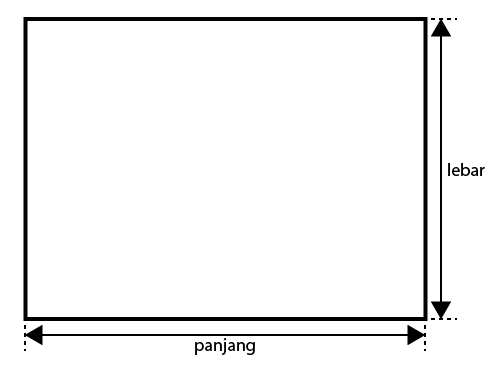
\includegraphics[scale=0.5]{model_ruangan}
	\caption[Pemodelan ruangan]{Pemodelan ruangan} 
	\label{fig:model_ruangan}
\end{figure}

%Dengan diketahuinya spesifikasi ruangan, maka akan diketahui daerah yang harus dicakup oleh kamera-kamera CCTV. Kamera-kamera CCTV akan ditempatkan dengan sedemian rupa sehingga seluruh daerah dapat tercakup. Untuk menyatakan posisi penempatan kamera CCTV, pemodelan masalah juga menggunakan sistem koordinat kertesius sehingga posisi penempatan dapat dinyatakan dalam koordinat x dan y. Dengan demikian, posisi penempatan kamera CCTV dapat dipahami lebih mudah.

\section{Kamera CCTV}
Hingga saat ini, sudah terdapat banyak jenis kamera CCTV yang diproduksi. Setiap kamera CCTV tersebut memiliki spesifikasinya masing-masing. Dalam permasalahan ini, terdapat 2 spesifikasi kamera CCTV yang digunakan, yaitu jarak pandang efektif dan besar sudut pandang. Gambar~\ref{fig:model_kamera} memodelkan kamera CCTV dengan kedua spesifikasi tersebut. Jarak pandang efektif adalah jarak pandang terjauh kamera CCTV untuk mengenali objek yang akan dipantau. Besar sudut pandang menunjukkan lebar pantauan kamera CCTV. Dalam permasalahan ini, jenis kamera CCTV yang digunakan hanya berjumlah 1 buah.

\begin{figure}[H]
	\centering  
	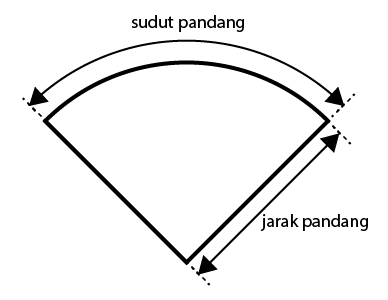
\includegraphics[scale=0.5]{model_kamera}
	\caption[Pemodelan kamera CCTV]{Pemodelan kamera CCTV} 
	\label{fig:model_kamera}
\end{figure}

\section{Penempatan Kamera CCTV}
Setelah ruangan dan kamera CCTV dimodelkan, langkah selanjutnya adalah memodelkan penempatan kamera-kamera CCTV. Setiap kamera CCTV dapat ditempatkan di mana saja selama posisinya berada di dalam ruangan. Selain posisi, penempatan juga melibatkan arah pandang kamera CCTV. Posisi dan arah pandang akan mempengaruhi daerah yang dapat dicakup oleh kamera CCTV. Untuk memodelkan penempatan ini, digunakan sistem koordinat kartesius sehingga posisi penempatan dinyatakan dalam bentuk koordinat (x,y). Arah padang kamera CCTV juga dapat dinyatakan dengan besar sudut arah pandang terhadap garis \(0^\circ\) yang melewati titik posisi kamera CCTV. Posisi dan arah pandang kamera CCTV dimodelkan seperti pada gambar~\ref{fig:model_penempatan_kamera} berikut ini.

\begin{figure}[H]
	\centering  
	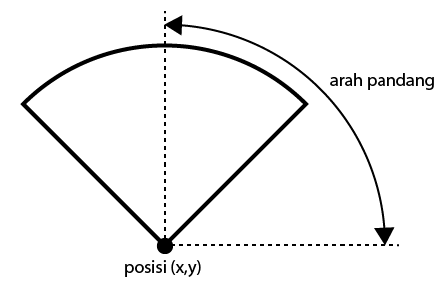
\includegraphics[scale=0.5]{model_penempatan_kamera}
	\caption[Pemodelan penempatan kamera CCTV]{Pemodelan penempatan kamera CCTV} 
	\label{fig:model_penempatan_kamera}
\end{figure}

\section{Daerah Cakupan Kamera CCTV}
Setiap penempatan kamera-kamera CCTV memiliki daerah yang dicakupnya masing-masing. Apabila terdapat 2 atau lebih kamera CCTV yang mencakup suatu daerah yang sama, maka daerah tersebut merupakan daerah irisan dari cakupan kamera-kamera CCTV tersebut. Daerah irisan ini memiliki bentuk yang tidak sederhana tetapi mudah untuk dipahami oleh manusia dengan penglihatan dan nalarnya. Berbeda dengan manusia, perangkat lunak tidak memiliki nalar untuk memahami kondisi daerah tersebut. Definisi daerah pun menjadi abstrak untuk dipahami ketika menyelesaikan permasalahan ini.

























